\uuid{QeZr}
\chapitre{Statistique}
\niveau{L2}
\module{Probabilité et statistique}
\sousChapitre{Tests d'hypothèses, intervalle de confiance}
\titre{Analyse de la précision d'un système d'arme}
\theme{statistiques, tests d'hypothèses}
\auteur{Maxime Nguyen}
\datecreate{2025-11-24}
\organisation{AMSCC}
\difficulte{4}
\contenu{
\texte{
	Dans le cadre de la qualification d'une section d'infanterie, on évalue la précision 
	du tir au FAMAS sur cible à 200 mètres. Le référentiel de l'armée de terre fixe 
	un écart-type maximal de $\sigma_0 = 8$ cm pour les impacts par rapport au centre 
	de la cible (tous tireurs confondus) pour qu'une section soit considérée comme opérationnelle.
	
	Un chef de section souhaite vérifier si sa section respecte ce standard. 
	Lors d'une séance de tir, 25 soldats effectuent chacun un tir, 
	et on mesure la distance de l'impact au centre de la cible (en cm). 
	
	\textbf{Distances observées (en cm) :}
	\begin{center}
		\begin{tabular}{ccccccccccc}
			5.2 & 12.3 & 8.7 & 6.5 & 15.1 & 9.2 & 7.4 & 11.8 & 4.9 & 13.6 & 9.8 \\
			4.1 & 11.2 & 7.8 & 13.5 & 6.9 & 10.5 & 8.3 & 14.2 & 5.7 & 7.2 & 10.1 \\
			8.9 & 12.5 & 6.3 & & & & & & & &
		\end{tabular}
	\end{center}
	
	\textbf{Statistiques calculées} (pour vérification) : 
	$\bar{x} = 9.23$ cm, $s^2 = 11.67$ cm$^2$, $s = 3.42$ cm
	
	On suppose que la distance des impacts suit une loi normale.
}
	\begin{enumerate}
		\item \question{ 
			Avant de réaliser les tests statistiques, visualiser les données :
			\begin{itemize}
				\item Représenter les distances par un histogramme ou un diagramme en boîte
				\item Cette représentation est-elle cohérente avec l'hypothèse de normalité ?
				\item Y a-t-il des valeurs aberrantes qui pourraient indiquer un problème 
				(tireur mal formé, incident de tir, etc.) ?
			\end{itemize}
		}

\indication{ Critère de Tukey : une valeur est aberrante si elle est en dehors de 
	$[Q1 - 1.5 \times IQR; Q3 + 1.5 \times IQR]$. }
		
\reponse{
	\textbf{Calculs des quartiles et statistiques descriptives :}
	
	En ordonnant les données :
	4.1, 4.9, 5.2, 5.7, 6.3, 6.5, 6.9, 7.2, 7.4, 7.8, 8.3, 8.7, 8.9, 
	9.2, 9.8, 10.1, 10.5, 11.2, 11.8, 12.3, 12.5, 13.5, 13.6, 14.2, 15.1
	
	\begin{itemize}
		\item Effectif : $n = 25$
		\item Minimum : 4.1 cm
		\item Q1 (25\%) : 6.7 cm (entre les valeurs 6.5 et 6.9)
		\item Médiane (50\%) : 8.9 cm (13\textsuperscript{e} valeur)
		\item Q3 (75\%) : 12.4 cm (entre les valeurs 12.3 et 12.5)
		\item Maximum : 15.1 cm
		\item Écart interquartile : IQR = Q3 - Q1 = 12.4 - 6.7 = 5.7 cm
	\end{itemize}
	
	\textbf{Recherche de valeurs aberrantes :}
	
	Critère de Tukey : une valeur est aberrante si elle est en dehors de 
	$[Q1 - 1.5 \times IQR; Q3 + 1.5 \times IQR]$
	
	$$[6.7 - 1.5 \times 5.7; 12.4 + 1.5 \times 5.7] = [-1.85; 20.95]$$
	
	Toutes les valeurs sont dans cet intervalle : \textbf{pas de valeur aberrante}.
	
	\textbf{Cohérence avec la normalité :}
	\begin{itemize}
		\item La distribution semble relativement symétrique autour de la médiane (8.9 cm)
		\item La médiane (8.9 cm) est très proche de la moyenne (9.23 cm), 
		ce qui suggère une distribution symétrique
		\item L'écart-type $s = 3.42$ cm représente environ 37\% de la moyenne, 
		ce qui est raisonnable
		\item Pas de valeurs extrêmes selon le critère de Tukey
		\item Distribution unimodale concentrée autour de 9 cm
		\item L'écart-type est nettement inférieur au standard requis (3.42 < 8 cm)
	\end{itemize}
	
	L'hypothèse de normalité semble acceptable pour ces données.
	
	\textbf{Diagramme en boîte (boîte à moustaches) :}
	
	\begin{center}
		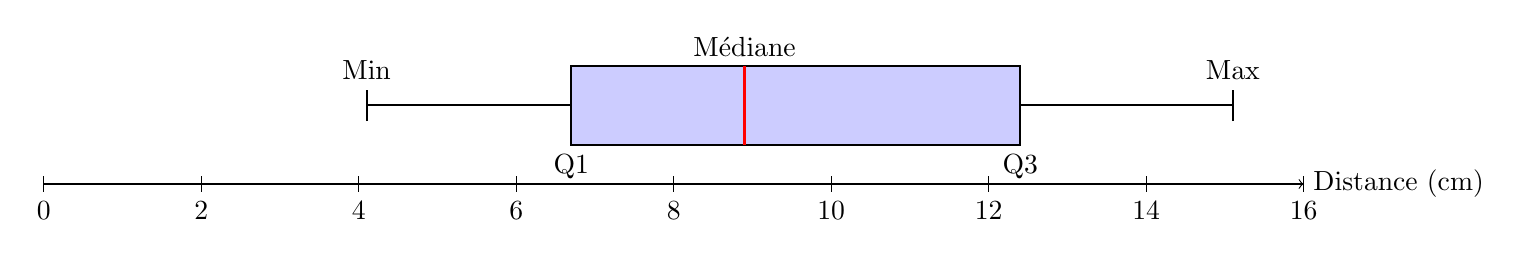
\begin{tikzpicture}
			\draw[->] (0,0) -- (16,0) node[right] {Distance (cm)};
			\foreach \x in {0,2,4,6,8,10,12,14,16}
			\draw (\x,0.1) -- (\x,-0.1) node[below] {\x};
			
			% Moustaches
			\draw[thick] (4.1,1) -- (6.7,1);
			\draw[thick] (12.4,1) -- (15.1,1);
			
			% Boîte
			\draw[thick,fill=blue!20] (6.7,0.5) rectangle (12.4,1.5);
			
			% Médiane
			\draw[very thick,red] (8.9,0.5) -- (8.9,1.5);
			
			% Marques
			\draw[thick] (4.1,0.8) -- (4.1,1.2) node[above] {Min};
			\draw[thick] (15.1,0.8) -- (15.1,1.2) node[above] {Max};
			\node[above] at (8.9,1.5) {Médiane};
			\node[below] at (6.7,0.5) {Q1};
			\node[below] at (12.4,0.5) {Q3};
		\end{tikzpicture}
	\end{center}
}

\indication{
	Avec un tableur :
	\begin{itemize}
		\item Trier les données : Sélectionner $\to$ Données $\to$ Trier
		\item Minimum : \texttt{=MIN(plage)} donne 4.1
		\item Q1 : \texttt{=QUARTILE.INCLURE(plage; 1)} donne 6.7
		\item Médiane : \texttt{=MEDIANE(plage)} ou \texttt{=QUARTILE.INCLURE(plage; 2)} donne 8.9
		\item Q3 : \texttt{=QUARTILE.INCLURE(plage; 3)} donne 12.4
		\item Maximum : \texttt{=MAX(plage)} donne 15.1
		\item IQR : \texttt{=Q3-Q1} donne 5.7
		\item Boîte à moustaches : Insertion $\to$ Graphique $\to$ Boîte à moustaches
	\end{itemize}
}
		
		\item \question{ 
			Le chef de section souhaite tester si sa section respecte le standard de l'armée.
			\begin{itemize}
				\item Formuler les hypothèses $H_0$ et $H_1$ de ce test
				\item Quel type de test doit-on utiliser ? (test bilatéral ou unilatéral ?)
				\item Justifier le choix de la statistique de test et donner sa loi sous $H_0$
			\end{itemize}
		}
		
		\reponse{
			\textbf{Formulation des hypothèses :}
			
			Le standard fixe $\sigma_0 = 8$ cm comme écart-type maximal. 
			On veut tester si la dispersion observée est conforme (ou meilleure) à ce standard.
			
			$$H_0 : \sigma^2 \leq \sigma_0^2 = 64 \text{ cm}^2 \quad \text{(section opérationnelle)}$$
			$$H_1 : \sigma^2 > \sigma_0^2 = 64 \text{ cm}^2 \quad \text{(précision insuffisante)}$$
			
			\textbf{Type de test :} Test unilatéral à droite, car on cherche à détecter 
			une dispersion \textit{trop grande} (problème opérationnel).
			
			\textbf{Statistique de test :}
			
			Pour tester une variance avec un échantillon de loi normale, on utilise :
			$$\chi^2 = \frac{(n-1)S^2}{\sigma_0^2}$$
			
			où $S^2 = \frac{1}{n-1}\sum_{i=1}^n (X_i - \bar{X})^2$ est la variance empirique.
			
			Sous $H_0$ (en prenant l'égalité $\sigma^2 = \sigma_0^2$), cette statistique suit 
			une loi du $\chi^2$ à $(n-1)$ degrés de liberté :
			$$\chi^2 \sim \chi^2_{n-1} = \chi^2_{24}$$
			
			\textbf{Justification :}
			
			Si $X_1, \ldots, X_n \stackrel{iid}{\sim} \mathcal{N}(\mu, \sigma^2)$, alors :
			$$\frac{(n-1)S^2}{\sigma^2} \sim \chi^2_{n-1}$$
		}
		
		\item \question{ 
			Au seuil de signification $\alpha = 5\%$, peut-on conclure que la section 
			respecte le standard de précision de l'armée de terre ?
		}
		
		\reponse{
			\textbf{Calcul de la statistique de test :}
			
			Avec $n = 25$, $s^2 = 11.67$ cm$^2$ et $\sigma_0^2 = 64$ cm$^2$ :
			
			$$\chi^2_{\text{obs}} = \frac{(n-1)s^2}{\sigma_0^2} = \frac{24 \times 11.67}{64} 
			= \frac{280.08}{64} = 4.376$$
			
			\textbf{Région critique :}
			
			Pour un test unilatéral à droite avec $\alpha = 5\%$ et 24 degrés de liberté, 
			on rejette $H_0$ si $\chi^2_{\text{obs}} > \chi^2_{0.95; 24}$.
			
			En consultant la table du $\chi^2$ : $\chi^2_{0.95; 24} = 36.415$
			
			\textbf{Décision :}
			
			$\chi^2_{\text{obs}} = 4.376 < 36.415$ : on se trouve dans la région d'acceptation.
			
			\textbf{On ne rejette pas $H_0$ au seuil $\alpha = 5\%$.}
			
			\textbf{Conclusion opérationnelle :}
			
			Au niveau de confiance de 95\%, les données ne permettent pas de rejeter l'hypothèse 
			que la section respecte le standard de précision de l'armée de terre. 
			La dispersion observée ($s \approx 3.42$ cm) est \textbf{significativement inférieure} 
			au standard requis ($\sigma_0 = 8$ cm).
			
			La section peut être considérée comme opérationnelle du point de vue 
			de la précision du tir.
		}
		
		\indication{
			Avec un tableur :
			\begin{itemize}
				\item Statistique : \texttt{=24*11.67/64} donne $4.376$
				\item Valeur critique : \texttt{=LOI.KHIDEUX.INVERSE(0.05; 24)} donne $36.415$
				\item $p$-valeur : \texttt{=1-LOI.KHIDEUX(4.376; 24; VRAI)} donne $\approx 0.9995$
			\end{itemize}
		}
		
		\item \question{ 
			Calculer un intervalle de confiance à 95\% pour l'écart-type $\sigma$ 
			de la population. Interpréter ce résultat dans le contexte militaire.
		}
		
		\reponse{
			\textbf{Intervalle de confiance pour $\sigma^2$ :}
			
			L'intervalle de confiance à $1-\alpha = 95\%$ pour $\sigma^2$ est :
			$$\left[\frac{(n-1)s^2}{\chi^2_{1-\alpha/2; n-1}}; \frac{(n-1)s^2}{\chi^2_{\alpha/2; n-1}}\right]$$
			
			Avec $n=25$, $s^2 = 11.67$, et les valeurs critiques du $\chi^2_{24}$ :
			\begin{itemize}
				\item $\chi^2_{0.975; 24} = 39.364$
				\item $\chi^2_{0.025; 24} = 12.401$
			\end{itemize}
			
			$$IC_{95\%}(\sigma^2) = \left[\frac{24 \times 11.67}{39.364}; \frac{24 \times 11.67}{12.401}\right] 
			= [7.12; 22.59] \text{ cm}^2$$
			
			\textbf{Intervalle de confiance pour $\sigma$ :}
			
			$$IC_{95\%}(\sigma) = [\sqrt{7.12}; \sqrt{22.59}] = [2.67; 4.75] \text{ cm}$$
			
			\textbf{Interprétation militaire :}
			
			Avec 95\% de confiance, l'écart-type réel de la section se situe entre 2.67 et 4.75 cm.
			
			\begin{itemize}
				\item Le standard de l'armée fixe $\sigma_0 = 8$ cm
				\item La borne supérieure de l'IC est 4.75 cm, \textbf{bien inférieure} à 8 cm
				\item Même dans le pire scénario (borne supérieure), la section reste largement 
				en deçà du seuil maximal
				\item Cela confirme que la section a une précision de tir \textbf{excellente}
				\item Le chef de section peut valider sa section comme opérationnelle 
				avec une grande confiance
			\end{itemize}
		}
		
		\indication{
			Avec un tableur :
			\begin{itemize}
				\item Borne inf : \texttt{=RACINE(24*11.67/LOI.KHIDEUX.INVERSE(0.025; 24))}
				\item Borne sup : \texttt{=RACINE(24*11.67/LOI.KHIDEUX.INVERSE(0.975; 24))}
			\end{itemize}
		}
		
		\item \question{ 			
			Le commandant de compagnie examine les résultats et fait la remarque suivante :
			
			\textit{« Votre section montre d'excellents résultats avec un écart-type de 3.4 cm, 
				bien meilleur que le standard de 8 cm. Cependant, je constate que la moyenne 
				des impacts est à 9.2 cm du centre. Ne faudrait-il pas aussi vérifier 
				que le tir n'est pas systématiquement décentré ? »}
			
			\begin{itemize}
				\item Le commandant a-t-il raison de s'interroger sur ce point ?
				\item Proposer et réaliser un test statistique pour vérifier 
				si le tir de la section présente un biais systématique 
				(hypothèse : le tir devrait être centré, donc $\mu = 0$)
				\item Que recommanderiez-vous au chef de section suite à cette analyse complète ?
			\end{itemize}
		}
		
		\reponse{
			\textbf{Pertinence de la remarque :}
			
			Le commandant a tout à fait raison. Un système d'arme peut être :
			\begin{itemize}
				\item \textbf{Précis} (faible dispersion, $\sigma$ petit) : c'est le cas ici
				\item \textbf{Juste} (pas de biais, impacts centrés sur la cible)
			\end{itemize}
			
			Un système précis mais biaisé reste problématique opérationnellement 
			(tous les tirs manquent le but dans la même direction).
			
			\textbf{Test de la moyenne :}
			
			On teste :
			$$H_0 : \mu = 0 \quad \text{(tir centré)}$$
			$$H_1 : \mu \neq 0 \quad \text{(tir biaisé)}$$
			
			Test bilatéral (le biais peut être dans n'importe quelle direction).
			
			Statistique de test (loi de Student car $\sigma$ inconnu) :
			$$t = \frac{\bar{x} - \mu_0}{s/\sqrt{n}} = \frac{9.23 - 0}{\sqrt{11.67}/\sqrt{25}} 
			= \frac{9.23}{3.416/5} = \frac{9.23}{0.683} = 13.51$$
			
			Sous $H_0$ : $t \sim \mathcal{T}_{24}$ (Student à 24 ddl).
			
			Pour $\alpha = 5\%$ bilatéral : $t_{0.975; 24} = 2.064$
			
			\textbf{Décision :}
			
			$|t_{\text{obs}}| = 13.51 > 2.064$ : \textbf{on rejette $H_0$}.
			
			La $p$-valeur est extrêmement faible (quasi nulle).
			
			\textbf{Conclusion :}
			
			Le tir de la section présente un \textbf{biais systématique très significatif} 
			d'environ 9.2 cm par rapport au centre.
			
			\textbf{Recommandations opérationnelles :}
			
			\begin{enumerate}
				\item \textbf{Diagnostic du biais :}
				\begin{itemize}
					\item Vérifier le réglage des hausses et des organes de visée
					\item Contrôler l'alignement des armes (armurerie)
					\item Analyser si le biais est identique pour tous les tireurs 
					(problème matériel) ou variable (problème de formation)
				\end{itemize}
				
				\item \textbf{Actions correctives :}
				\begin{itemize}
					\item Faire réviser les armes par l'armurerie
					\item Refaire un tir de réglage après correction
					\item Vérifier les conditions de tir (vent latéral ? position de tir ?)
				\end{itemize}
				
				\item \textbf{Qualification :}
				\begin{itemize}
					\item La section est \textbf{précise} (bonne dispersion)
					\item Mais elle n'est \textbf{pas juste} (biais significatif)
					\item Après correction du biais, elle devrait être pleinement opérationnelle
				\end{itemize}
			\end{enumerate}
		
		}
		
		\indication{
			Avec un tableur :
			\begin{itemize}
				\item Écart-type : \texttt{=RACINE(11.67)} donne $3.416$ cm
				\item Statistique $t$ : \texttt{=9.23/(3.416/RACINE(25))} donne $13.51$
				\item Valeur critique : \texttt{=LOI.STUDENT.INVERSE.BILATERALE(0.05; 24)} donne $2.064$
				\item $p$-valeur : \texttt{=LOI.STUDENT.BILATERALE(13.51; 24)} donne $\approx 4.6 \times 10^{-13}$
			\end{itemize}
		}
		
		\item \question{
			Un officier du bureau emploi propose de comparer cette section avec une autre section 
			de la même compagnie qui a obtenu les résultats suivants (20 tireurs) : 
			$\bar{y} = 8.1$ cm, $s_y^2 = 15.3$ cm$^2$.
			
			Les deux sections ont-elles le même niveau de précision ? 
			Réaliser un test de comparaison de variances au seuil de 5\%.
		}
		
		\reponse{
			\textbf{Test de comparaison de deux variances (test de Fisher) :}
			
			On teste :
			$$H_0 : \sigma_1^2 = \sigma_2^2 \quad \text{(même précision)}$$
			$$H_1 : \sigma_1^2 \neq \sigma_2^2 \quad \text{(précisions différentes)}$$
			
			Statistique de test :
			$$F = \frac{s_2^2}{s_1^2} = \frac{15.3}{11.67} = 1.311$$
			
			(On place la plus grande variance au numérateur pour avoir $F \geq 1$)
			
			Sous $H_0$ : $F \sim \mathcal{F}(n_2-1, n_1-1) = \mathcal{F}(19, 24)$ 
			(loi de Fisher).
			
			Pour un test bilatéral à $\alpha = 5\%$, on compare $F_{\text{obs}}$ avec 
			$F_{0.975; 19, 24}$ et $F_{0.025; 19, 24}$.
			
			En pratique, pour un test bilatéral avec $F > 1$, on compare avec $F_{1-\alpha/2}$ :
			$$F_{0.975; 19, 24} \approx 2.41$$
			
			\textbf{Décision :}
			
			$F_{\text{obs}} = 1.311 < 2.41$ : \textbf{on ne rejette pas $H_0$}.
			
			\textbf{Conclusion :}
			
			Au seuil de 5\%, on ne peut pas conclure à une différence significative 
			de précision entre les deux sections. Les écarts observés peuvent être 
			attribués à la variabilité d'échantillonnage.
			
			\textbf{Interprétation opérationnelle :}
			
			Les deux sections ont un niveau de précision comparable. 
			Le commandant de compagnie peut considérer que la formation au tir 
			est homogène entre les sections.
		}
		
		\indication{
			Avec un tableur :
			\begin{itemize}
				\item Statistique $F$ : \texttt{=15.3/11.67} donne $1.311$
				\item Valeur critique : \texttt{=LOI.F.INVERSE(0.025; 19; 24)} donne $\approx 2.41$
				\item $p$-valeur : \texttt{=2*MIN(LOI.F(1.311; 19; 24; VRAI); 1-LOI.F(1.311; 19; 24; VRAI))}
			\end{itemize}
		}
	\end{enumerate}
}